
\section{Common Spatial Patternとその派生手法}
\label{sec:CSP}
運動想起型BCIにおいて非常に活発に用いられている``Common Spatial Pattern(CSP)''は1990年にZoltan\cite{CSP1990}により提案されてから、
数々の派生手法が生み出されてきた\cite{CSP1999,cvscsp,fbcsp,csssp,csp_eigen,カーネルCSP,正則化CSP}。
このセクションではCSPの基本的な概要と、BCIに適した形で発展してきたCSPの派生手法について述べる。

\subsection{脳波信号の定式化}
これまで多次元の信号を\(x(t)\in \mathbb R^D\)と表記し、連続時間信号として扱ってきた。
しかし、通常は計測された脳波はコンピュータで処理するために
離散時間信号\(x_n \in \mathbb R^D\)に変換される。
従って、以降、脳波信号を離散時間信号として取り扱う。
また、運動想起時の脳波信号を計測する際には、
被験者に対して定められたタイムスケジュールで運動想起を行うように指示がなされる。
例として64個の電極を用い、サンプリング周波数100Hzで10秒間の計測を行った場合、
計測された運動想起1回分の脳波信号は\(X \in \mathbb{R}^{64 \times 1000}\)
と表すことができる。従って、以降統一のため、\(M\)を電極の個数、
\(N\)を計測時間点数とした場合の脳波信号を以下で定義する\begin{equation}
    X =(x_1, \cdots, x_N)\in \mathbb{R}^{M \times N}\    
\end{equation}


運動想起を\(K\)回行った場合には、\(K\)個の\(X\)が得られる。
通常は運動想起時の脳波を数個から数十個集め、統計的な指標を元に有用な特徴量を抽出する。
CSPは運動想起BCIに対して極めて有効に働くとされている特徴量抽出手法である。


\subsection{Common Spatial Pattern(CSP)}
\label{subsec:CSP}
CSPは複数の電極で計測されることが一般的である脳波に対して、
適切な電極の重み付けを行うことで、重要な頭皮領域の脳波を取り出す手法である。
CSPを脳波に用いる際は、脳波信号\(X\)を直接扱うのではなく、何らかの前処理を施した信号\(\hat{X} = {\cal H}(X) \)を用いる。
通常、\(\cal H\)には、運動想起に関連のある周波数帯域のみを通過させるバンドパスフィルタを用いる(図\ref{fig:CSP})。
\begin{figure}
    \centering
    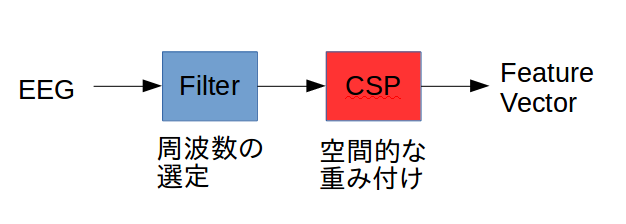
\includegraphics[width=12cm]{images/CSP.png}
    \caption{CSPの利用方法}
    \label{fig:CSP}
\end{figure}
バンドパスフィルタ通過後の脳波信号を以下のように表記する。
\begin{equation}
    \hat X = \left( \hat x_1,\cdots,\hat x_N \right) \in \mathbb{R}^{M \times N}
\end{equation}
\(\hat x_i \in \mathbb R^M\)における添字\(i\)はサンプル時刻の添え字である。
CSPでは、新たな基底\(w\in \mathbb R^M\)にバンドパスフィルタ通過後の脳波信号を射影し、
スカラー時間信号である\(z=w^T\hat X\in \mathbb R^N\)を抽出する。この時の\(w\)の決め方を以下に記す。

まず\(\hat X\)を基底\(w\)に射影した際の時間分散\(\sigma^2 (\hat X, w)\)を以下で定義する。
\begin{equation}
    \sigma^2 (\hat X, w)  = \frac{1}{N}\sum_{i=1}^N \left|w^T \left(\hat x_i - \frac{1}{N} \sum_{j=1}^N \hat x_j \right) \right|^2
    \label{timevar}
\end{equation}
ここで計測された複数個の\(\hat X\)は必ず集合\(C_1\)か\(C_2\)のいずれか一方に属するとし、
\(C_1 \cap C_2 = \phi \)であるとする。
CSPでは、ベクトル\(w \in \mathbb {R}^M\)を新たな基底とした電極空間において、
一方のクラスに属する信号\(\hat X \in {C_d}\)についての時間分散(\ref{timevar})が最大となるように、\(w\)を決める。
これは以下の最大化問題によって定式化される。
\begin{equation}
    \begin{aligned}
    & \max_w
    & & \mathbb E_{X \in C_1} \left[\sigma^2 (\hat X, w) \right] \\
    & \text{s.t.}
    & &  \sum_{d=1,2} \mathbb E_{X \in C_d} \left[\sigma^2 (\hat X, w) \right] = 1
    \end{aligned}
    \label{eq:objcsp}
\end{equation}
最大化問題(\ref{eq:objcsp})を解いて得られる\(w_{csp}\)は、
クラス\(C_1\)に属する脳波の分散を最大化するような基底である。
一方で、制約条件によって2つのクラスの分散の和が\(1\)であるとされているため、
自動的にクラス\(C_2\)に属する脳波の分散を最小化する基底ともなる。
すなわち\(w_{csp}\)によって得られるスカラー信号は一方のクラスの信号のみを増幅させ、他方を減衰させる働きをする。
(\ref{eq:objcsp})は更に以下で定式化することができる。
\begin{equation}
    \begin{aligned}
    & \max_w
    & & w^T\Sigma_1 w \\
    & \text{s.t.}
    & &  w^T(\Sigma_1+\Sigma_2)w = 1
    \end{aligned}
    \label{eq:objcsp2}
\end{equation}
ここで
\begin{equation}
    \Sigma_i = \mathbb E_{X\in C_i}\left[\frac{\hat X \hat X^T}{{\rm tr}(\hat X \hat X^T)}\right]
\end{equation}
である。この問題の解はラグランジュ法によって解析的に求めることが可能である。
簡単な計算によって(\ref{eq:objcsp2})は以下の一般化固有値問題に帰着される\cite{csp_eigen}。
\begin{equation}
    \Sigma_1w = \lambda(\Sigma_1+\Sigma_2)w
\end{equation}
この一般化固有値問題は右辺の\(\Sigma_1+\Sigma_2\)が正則であれば、
その逆行列を両辺左から掛けることで普通の固有値問題に変形できる。

一般化固有値問題が解けた時のM個の固有値を\(\lambda_1 \geq \lambda_2 \geq \cdots \geq \lambda_M\)とする。
また、\(\lambda_i\)に属する固有ベクトルを\(w^{(i)}\)とする。
このとき最適化問題の解に相当するのは\(w^{(1)}\)であり、
\(C_1\)に属する脳波を増幅し、\(C_2\)に属する脳波を減衰させたスカラー信号を獲得できる。
一方で\(w^{(M)}\)は\(C_1\)に属する脳波を減衰し、\(C_2\)に属する脳波を増幅させたスカラー信号を獲得できる。
従って通常は、\(w^{(1)},w^{(M)}\)の固有ベクトルを対で用いる。同様に\(w^{(2)},w^{(M-1)}\)を対で取り出して4つの固有ベクトルを用いることもできる。
一般に\(2m(<M)\)個の固有ベクトルを使うこととすれば、特徴量\(\sigma^2(\hat X,w^{(i)})\)を\(2m\)個準備することができる。
ここで単に\(z=w^{(i)}\hat X\)を用いないのは、CSPによって得られる特徴量は振幅に大きな違いがあるためである。
通常はCSPによって獲得される特徴量\(y\)は以下の形式となる。
\begin{equation}
    y = (\sigma^2(\hat X,w^{(1)}), \cdots, \sigma^2(\hat X,w^{(m)}), \cdots, \sigma^2(\hat X,w^{(M-m+1)}), \cdots, \sigma^2(\hat X,w^{(M)}))^T
\end{equation}
あるいは\(y=(y_1, \cdots, y_{2m})\)に対して以下のような変換を行った特徴量\(f\)を使う。
\begin{eqnarray}
    f_i &=& \log \left( \frac{y_i}{\sum_{i=1}^{2m}y_i} \right) \nonumber \\
    f &=& (f_1, \cdots, f_{2m})^T 
\end{eqnarray}
また\(m=1,2\)が多くのCSPの応用研究で使われており、\(m\)を増やしてもBCIの性能向上には繋がらないことが報告されている\cite{cvscsp}。
% 行列\(W_{csp}\)を
% \begin{equation}
%     W_{csp}=(w^{(1)},\cdots,w^{(m)},\cdots,w^{(M-m+1)},\cdots,w^{(M)}) \in \mathbb R^{2m \times M}
% \end{equation}
% によって構成し、脳波信号\(X \in \mathbb R^{M\times N}\)から以下の変換によって\(Z \in \mathbb R^{2m \times N}\)を獲得できる。
% \begin{equation}
%     Z = W_{csp}^TX
% \end{equation}
% ここで通常は\(Z=(z_1, z_2, \cdot, z_N)\)の成分毎の時間分散を特徴量とする。
% \(Z\)の脳波のパワーを評価することが可能となる。

\begin{figure}
    \centering
    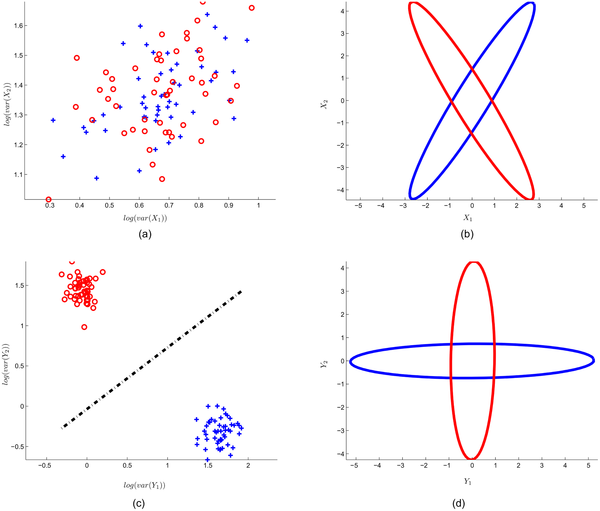
\includegraphics[width=12cm]{images/apple.png}
    \caption{林檎の図}
\end{figure}
  

\subsection{Common Sparse Spatio Spectral Pattern(CSSSP)}
CSPではバンドパスフィルタ\(\cal H\)通過後の信号を扱ったため、
バンドパスフィルタの設計を終えてからでなければCSPの問題を解くことができない。
従って、あるバンドパスフィルタを通過した脳波に対して、最適化問題を解いているに過ぎなく、
バンドパスフィルタ自体が適切であったかに関しては一切述べられない。
このことによって生じる問題点に関しては、更に詳しく後述する。
CSSSPの主なモチベーションはバンドパスフィルタの設計をCSPの問題の中に取り込むことである\cite{csssp}。

まず脳波信号\(X = \left[ x_1, \cdots, x_N \right] \in \mathbb{R}^{M \times N}\)に対して、
観測時間点を\(\tau\ > 0\)だけずらした\(X_{\tau} = \left( x_{1+\tau}, \cdots, x_{N+\tau} \right) \in \mathbb{R}^{M \times N}\)を考える。
ここで$\tau = 1,\ldots,T$である。
更にクラス\( C_d \)に属する\( X \)に関して各\(\tau\)毎に、
\begin{equation}
    \Sigma_{d}^{\tau} = \mathbb E_{X \in C_d} \left[ XX_{\tau}^T + X_{\tau}X^T \right]
\end{equation}
を定義する。ただし\(\tau=0\)のとき\( \Sigma_{d}^{0} = \mathbb E_{X \in C_d} \left[XX^T \right] \)とする。
更に、\(T\)個の要素を持つ係数ベクトル$b=(b_1,b_2,\ldots,b_T)^T$とする。
ここでCSSSPの最適化問題は以下で表現される。
\begin{equation}
    \begin{aligned}
        & \max_{b_2,\ldots,b_T} \max_{w}
        & & w^T \left\{ \sum_{\tau = 0}^{T-1} \left( \sum_{j=1}^{T-\tau} b_j b_{j+\tau} \right) \Sigma_1^{\tau} \right\} w - \frac{\alpha}{T}|b|_1 \\
        & \text{subject to}
        & &  w^T \left[\sum_{\tau = 0}^{T-1} \left\{ \sum_{j=1}^{T-\tau}b_jb_{j+\tau} \right\} (\Sigma_1^{\tau} + \Sigma_2^{\tau}) \right] w = 1
    \end{aligned}
    \label{eq:csssp}
\end{equation}
この最適化問題の目的関数第1項は\(b\)をFIRフィルタ\(f\)の係数ベクトルとした場合に、
\(f\)を通過後の脳波\(X\)に対してCSPの最適化問題を適用していることに相当する。
従ってCSSSPでは空間重みベクトル\(w \in \mathbb R^M\)と次数が\(T\)のFIRフィルタのフィルタ係数\(b\)を同時に評価することが可能である(図\ref{fig:CSSSP})。
\begin{figure}
    \centering
    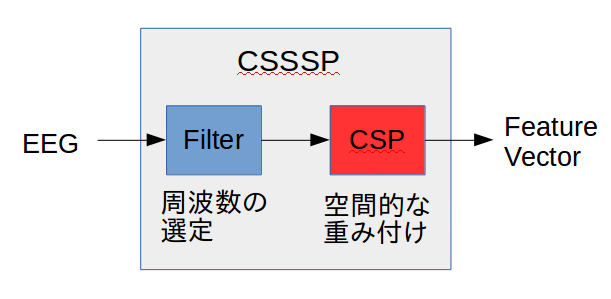
\includegraphics[width=9cm]{images/CSSSP.png}
    \caption{CSSSPの働き}
    \label{fig:FBCSP}
\end{figure}
目的関数における第二項は正則化項であり、$\alpha$はハイパーパラメータである。
この正則化によってFIRフィルタの系列ベクトルに対してスパース性が要請され、
フィルタリングに用いられる時系列点数は必要最小限に抑えられる。
このことによりFIRフィルタが必要以上に複雑になることが避けられる。
解析的に解くことは困難であるため、勾配法あるいはニュートン法を用いた直線探索によって数値的に解を得る。


\subsection{Filter Bank Common Spatial Pattern(FBCSP)}
CSSSPはFIRフィルタの設計をCSPの最適化問題に含むことで、バンドパスフィルタとCSPの同時最適化の定式化に成功した。
しかし、CSSSPによって求まる特徴量はフィルタ係数\(b\)を持つFIRフィルタを通過し、
変換行列\(W^T\)のCSPによって変換された脳波信号であり、
ある1つの周波数領域のみしか考慮されていないこととなる。
CSSSPを解いて得られるフィルタ係数\(b\)は最適化問題の解であるが、
必ずしもそのフィルタ係数のみを用いることが最良であるとは言い難い。
なぜなら、運動想起を行う際にはその身体部位に応じて特徴的な変動を持つ周波数領域は異なっているためである。
例えば左手の運動想起時と下肢の運動想起時では重要な周波数帯域が異なり、
CSSSPの解がいずれかの情報を失ってしまっている可能性が考えられる。FBCSPはこのような問題の解決を図る手法である\cite{fbcsp}。

まず、FBCSPではバンドパスフィルタバンク\(\{ {\cal H}_1, \ldots, {\cal H}_F \}\)を定義する。
このバンドパスフィルタバンクは1つ1つのフィルタ\({\cal H}_f\)が異なる周波数領域を通過させるように設計される。
各バンドパスフィルタを通過した\(\hat X_f = {\cal H}_f(X)\)に対して、
それぞれCSPの問題を解くことで各周波数領域における空間的な特徴量を獲得することが可能となる。
\({\hat X}_f\)に対してCSPによって取り出した特徴量を\(f_f\)とすれば、最終的な特徴ベクトル\(f\)は
\begin{equation}
    f = (f_1^T,\cdots, f_F^T)^T
\end{equation}
であり、単に各周波数帯域のCSPによる特徴量を連結したベクトルとなる。
ただしCSSSPとは異なり、CSPとバンドパスフィルタの同時最適化を行ってはいない。
従って、特徴ベクトル\(f\)のいずれの要素が重要であるか、すなわちいずれの周波数帯域が重要であるか
に関しての最適化は行われておらず、あくまで複数の周波数帯域において
それぞれの最適な電極の重み付けをCSPによって獲得したにすぎない。
そのため、FBCSPによって得られた特徴量から更に特徴量を抽出する手法が別途用いられる図\ref{fig:FBCSP}。
また、FBCSP後の特徴量の選定を行う方法として相互情報量を用いた手法が提案されている\cite{fbcspBCICOMPE}。
\begin{figure}
    \centering
    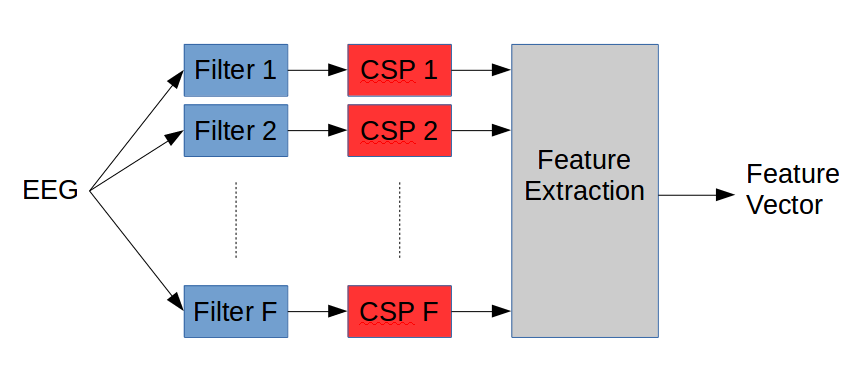
\includegraphics[width=12cm]{images/FBCSP.png}
    \caption{FBCSPを用いた処理の全体像}
    \label{fig:FBCSP}
\end{figure}